\documentclass[tikz,border=4pt]{standalone}
\pdfinfoomitdate=1
\pdftrailerid{}
\pdfsuppressptexinfo=-1
\usepackage{pgfplots}
\usepgfplotslibrary{groupplots}
\usetikzlibrary{arrows.meta,calc}
\pgfplotsset{compat=1.18}
\definecolor{guideblue}{RGB}{30,113,164}
\definecolor{guideteal}{RGB}{42,157,143}
\definecolor{guideorange}{RGB}{202,104,42}
\definecolor{guidegold}{RGB}{225,174,51}
\definecolor{guidegray}{RGB}{103,112,119}
\begin{document}
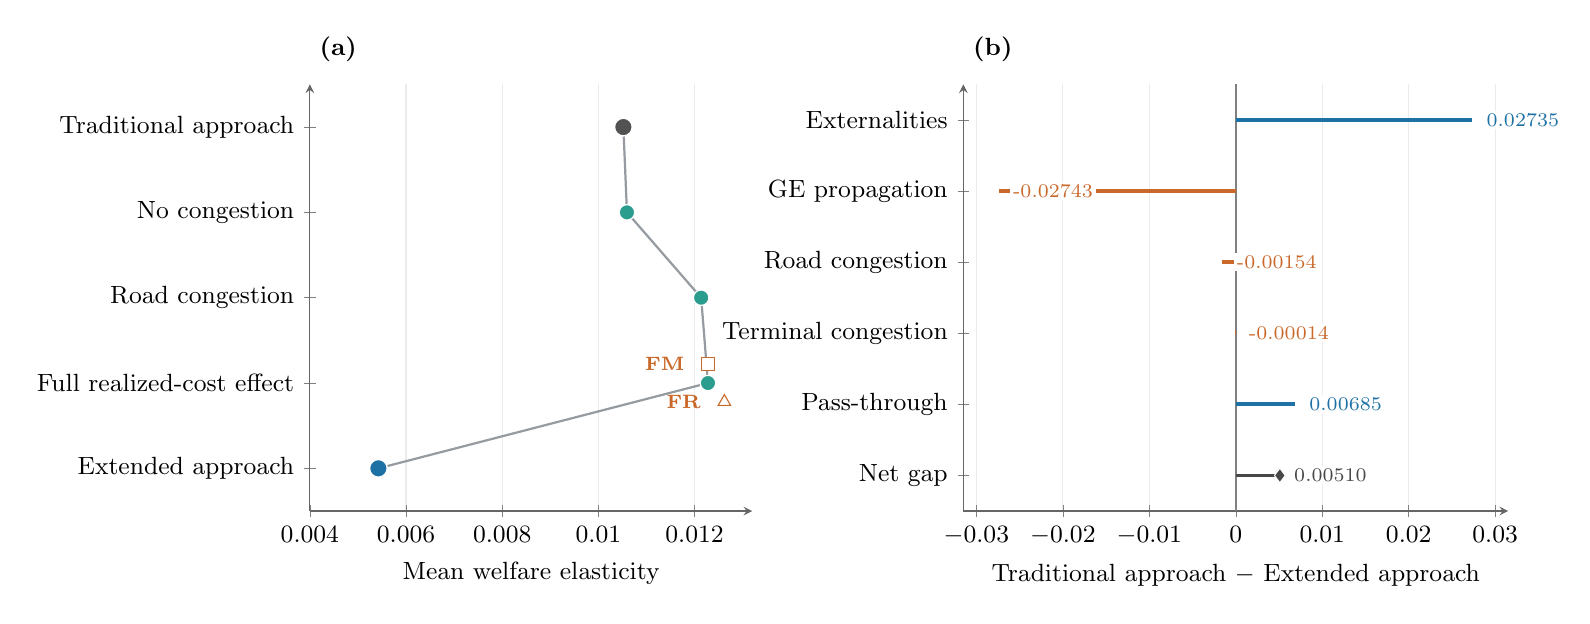
\begin{tikzpicture}
\begin{axis}[name=ladder,width=7.2cm,height=7.0cm,at={(0cm,0cm)},anchor=south west,xmin=0.004,xmax=0.0132,ymin=0.5,ymax=5.5,ytick={1,2,3,4,5},yticklabels={Extended approach,Full realized-cost effect,Road congestion,No congestion,Traditional approach},axis lines=left,axis line style={black!60},xmajorgrids=true,grid style={black!8},xlabel={Mean welfare elasticity},tick label style={font=\small},label style={font=\small},scaled ticks=false,xticklabel style={/pgf/number format/fixed,/pgf/number format/precision=3},clip=false]
\addplot[guidegray!70,line width=0.8pt] coordinates {
(0.010520000000,5)
(0.010594295706,4)
(0.012137714881,3)
(0.012279361886,2)
(0.005424755948,1)
};
\addplot[only marks,mark=*,mark size=2.8pt,draw=white,line width=0.45pt,fill=guideteal] coordinates {
(0.010594295706,4)
(0.012137714881,3)
(0.012279361886,2)
};
\addplot[only marks,mark=*,mark size=3.2pt,draw=white,line width=0.5pt,fill=black!68] coordinates {(0.010520000000,5)};
\addplot[only marks,mark=*,mark size=3.2pt,draw=white,line width=0.5pt,fill=guideblue] coordinates {(0.005424755948,1)};
\addplot[only marks,mark=square*,mark size=2.3pt,draw=guideorange,fill=white] coordinates {(0.012280243510,2.22)};
\addplot[only marks,mark=triangle*,mark size=2.6pt,draw=guideorange,fill=white] coordinates {(0.012620644517,1.78)};
\node[anchor=east,font=\scriptsize\bfseries,text=guideorange] at (axis cs:0.012280243510,2.22) [xshift=-5pt] {FM};
\node[anchor=east,font=\scriptsize\bfseries,text=guideorange] at (axis cs:0.012620644517,1.78) [xshift=-5pt] {FR};
\node[anchor=south west,font=\small\bfseries] at (rel axis cs:0,1.03) {(a)};
\end{axis}
\begin{axis}[width=8.5cm,height=7.0cm,at={(8.3cm,0cm)},anchor=south west,xmin=-0.0315,xmax=0.0315,ymin=0.5,ymax=6.5,ytick={1,2,3,4,5,6},yticklabels={Net gap,Pass-through,Terminal congestion,Road congestion,GE propagation,Externalities},axis lines=left,axis line style={black!60},xmajorgrids=true,grid style={black!8},xlabel={Traditional approach $-$ Extended approach},tick label style={font=\small},label style={font=\small},scaled ticks=false,xticklabel style={/pgf/number format/fixed,/pgf/number format/precision=2},clip=false]
\draw[black!50,line width=0.7pt] (axis cs:0,0.5)--(axis cs:0,6.5);
\draw[guideblue,line width=1.35pt] (axis cs:0,6)--(axis cs:0.027352000000,6);
\addplot[only marks,mark=circle*,mark size=2.6pt,draw=white,line width=0.35pt,fill=guideblue] coordinates {(0.027352000000,6)};
\node[anchor=west,font=\scriptsize,text=guideblue,fill=white,inner sep=1pt] at (axis cs:0.027352000000,6) [xshift=4pt] {0.02735};
\draw[guideorange,line width=1.35pt] (axis cs:0,5)--(axis cs:-0.027426295706,5);
\addplot[only marks,mark=circle*,mark size=2.6pt,draw=white,line width=0.35pt,fill=guideorange] coordinates {(-0.027426295706,5)};
\node[anchor=west,font=\scriptsize,text=guideorange,fill=white,inner sep=1pt] at (axis cs:-0.027426295706,5) [xshift=4pt] {-0.02743};
\draw[guideorange,line width=1.35pt] (axis cs:0,4)--(axis cs:-0.001543419174,4);
\addplot[only marks,mark=circle*,mark size=2.6pt,draw=white,line width=0.35pt,fill=guideorange] coordinates {(-0.001543419174,4)};
\node[anchor=west,font=\scriptsize,text=guideorange,fill=white,inner sep=1pt] at (axis cs:-0.001543419174,4) [xshift=4pt] {-0.00154};
\draw[guideorange,line width=1.35pt] (axis cs:0,3)--(axis cs:-0.000141647005,3);
\addplot[only marks,mark=circle*,mark size=2.6pt,draw=white,line width=0.35pt,fill=guideorange] coordinates {(-0.000141647005,3)};
\node[anchor=west,font=\scriptsize,text=guideorange,fill=white,inner sep=1pt] at (axis cs:-0.000141647005,3) [xshift=4pt] {-0.00014};
\draw[guideblue,line width=1.35pt] (axis cs:0,2)--(axis cs:0.006854605938,2);
\addplot[only marks,mark=circle*,mark size=2.6pt,draw=white,line width=0.35pt,fill=guideblue] coordinates {(0.006854605938,2)};
\node[anchor=west,font=\scriptsize,text=guideblue,fill=white,inner sep=1pt] at (axis cs:0.006854605938,2) [xshift=4pt] {0.00685};
\draw[black!72,line width=1.35pt] (axis cs:0,1)--(axis cs:0.005095244052,1);
\addplot[only marks,mark=diamond*,mark size=2.6pt,draw=white,line width=0.35pt,fill=black!72] coordinates {(0.005095244052,1)};
\node[anchor=west,font=\scriptsize,text=black!72,fill=white,inner sep=1pt] at (axis cs:0.005095244052,1) [xshift=4pt] {0.00510};
\node[anchor=south west,font=\small\bfseries] at (rel axis cs:0,1.03) {(b)};
\end{axis}
\end{tikzpicture}
\end{document}
